\documentclass{beamer}

\usefonttheme{professionalfonts} % using non standard fonts for beamer
\usefonttheme{serif} % default family is serif

\usepackage{enumitem}
\setitemize{label=\usebeamerfont*{itemize item}%
  \usebeamercolor[fg]{itemize item}
  \usebeamertemplate{itemize item}}

\usepackage{hyperref}
\usepackage{booktabs}
\usepackage{xfp}
\usepackage{graphicx}
\def\Put(#1,#2)#3{\leavevmode\makebox(0,0){\put(#1,#2){#3}}}
\usepackage{colortbl}
\usepackage{tikz}
\usepackage{amssymb}
\usepackage{enumerate}
\usepackage{arydshln}
\usepackage{algorithm}
\usepackage{algpseudocode}
\usepackage{subcaption} %to have subfigures available

\usepackage[absolute,overlay]{textpos}

\colorlet{lightred}{red!25}
\colorlet{lightgreen}{green!25}
\beamertemplatenavigationsymbolsempty

\newcommand\blfootnote[1]{%
  \begingroup
  \renewcommand\thefootnote{}\footnote{#1}%
  \addtocounter{footnote}{-1}%
  \endgroup
}

\makeatletter

%% Textclass specific LaTeX commands.
\newcommand\makebeamertitle{\frame{\maketitle}}%
\AtBeginDocument{%
  \let\origtableofcontents=\tableofcontents
  \def\tableofcontents{\@ifnextchar[{\origtableofcontents}{\gobbletableofcontents}}
  \def\gobbletableofcontents#1{\origtableofcontents}
}
%% User specified LaTeX commands.
\usetheme{Malmoe}
\useoutertheme{infolines}
\addtobeamertemplate{headline}{}{\vskip2pt}
\setbeamercovered{transparent}

\title[PFlock report]{PFLOCK Report}
\author[AC]{Andres Calderon}
\institute[UCR]{University of California, Riverside}
\makeatother

%%%%%%%%%%%%%%%%%%%%%%%%%%%%%%%%%%%%%%
%% Main document
%%%%%%%%%%%%%%%%%%%%%%%%%%%%%%%%%%%%%%
\begin{document}
\makebeamertitle
\newif\iflattersubsect

\AtBeginSection[] {
    \begin{frame}<beamer>
    \frametitle{Outline} 
    \tableofcontents[currentsection]  
    \end{frame}
    \lattersubsectfalse
}

\AtBeginSubsection[] {
    \begin{frame}<beamer>
    \frametitle{Outline} 
    \tableofcontents[currentsubsection]  
    \end{frame}
}

\begin{frame}{Still slow for dense cells}
    \centering
    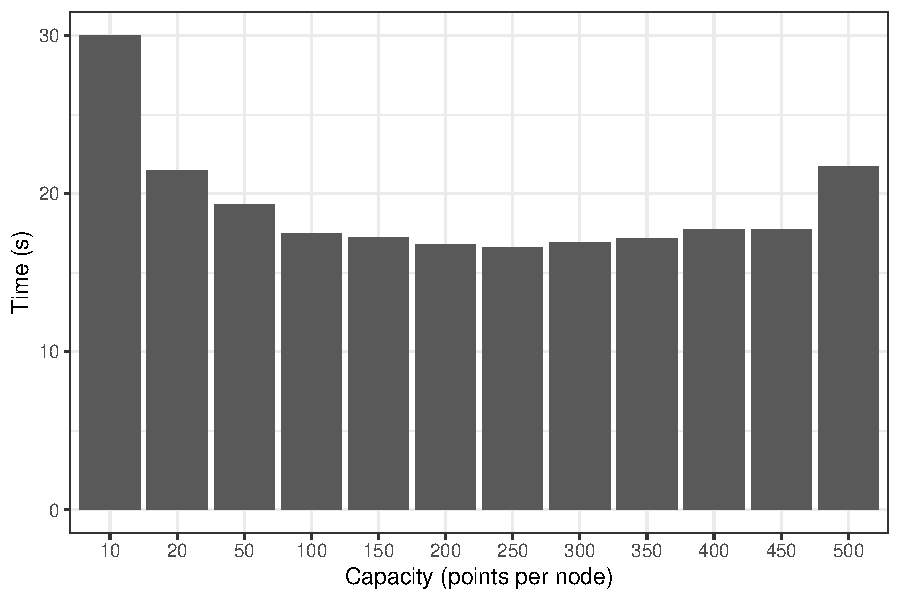
\includegraphics[width=0.7\textwidth]{figures/Capacity/capacity}
\end{frame}

\begin{frame}{Still slow for dense cells}
        \centering
        \begin{tikzpicture}
                \node[anchor=south west,inner sep=0] at (0,0) {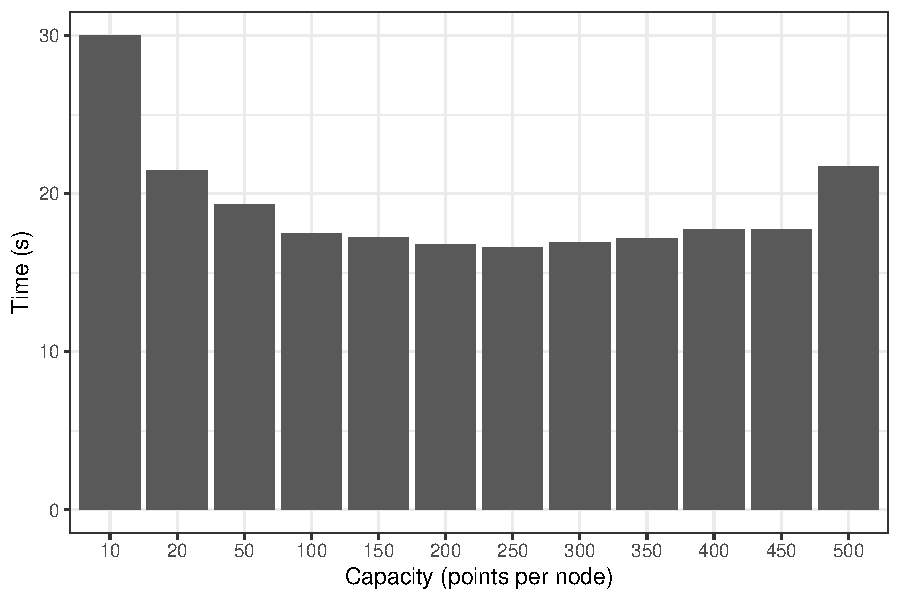
\includegraphics[width=0.7\textwidth]{figures/Capacity/capacity}};
                \draw<1>[red,ultra thick,rounded corners] (4.4,0.75) rectangle (5.2,3.4);
        \end{tikzpicture}
\end{frame}


\begin{frame}{Change title...}
        \centering
        \begin{tikzpicture}
                \foreach \i in {1,...,8} {
                        \def\j{\fpeval{9000 - \i * 1000}}
                        \node<\i>[] at (5,-0.25) {density=\j};
                        \node<\i>[anchor=south west,inner sep=0] at (0,0) {
                                \includegraphics[width=1.25\textheight]{figures/Cells/Cells\j}
                        };
                }
        \end{tikzpicture}
\end{frame}

\begin{frame}{Detecting maximal duplicates, subsets and supersets}
        {Sum of time for each candidate to be evaluated...}
        \centering
        \begin{minipage}{0.49\textwidth}
                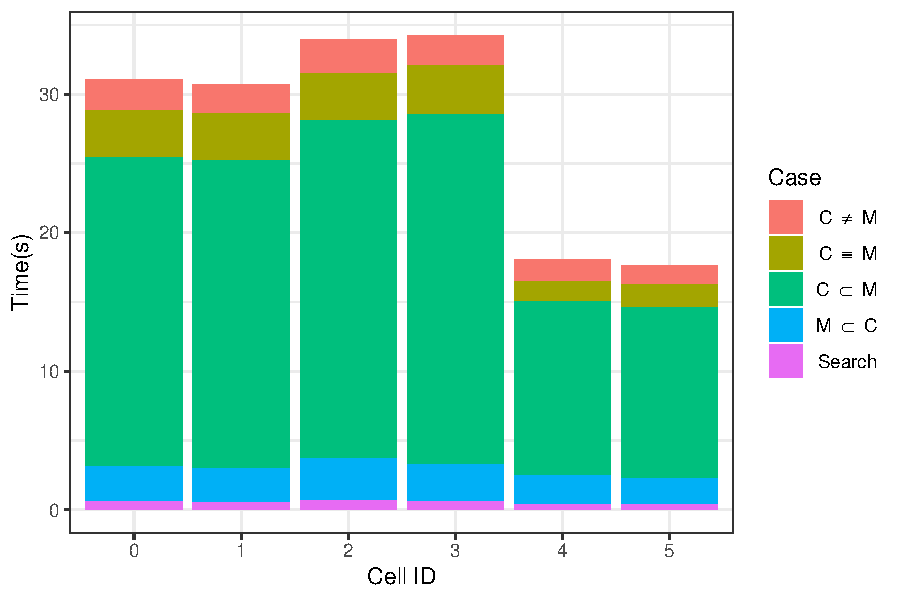
\includegraphics[width=\textwidth]{figures/Maximals/performanceBySum1}
        \end{minipage} %
        \begin{minipage}{0.49\textwidth}
                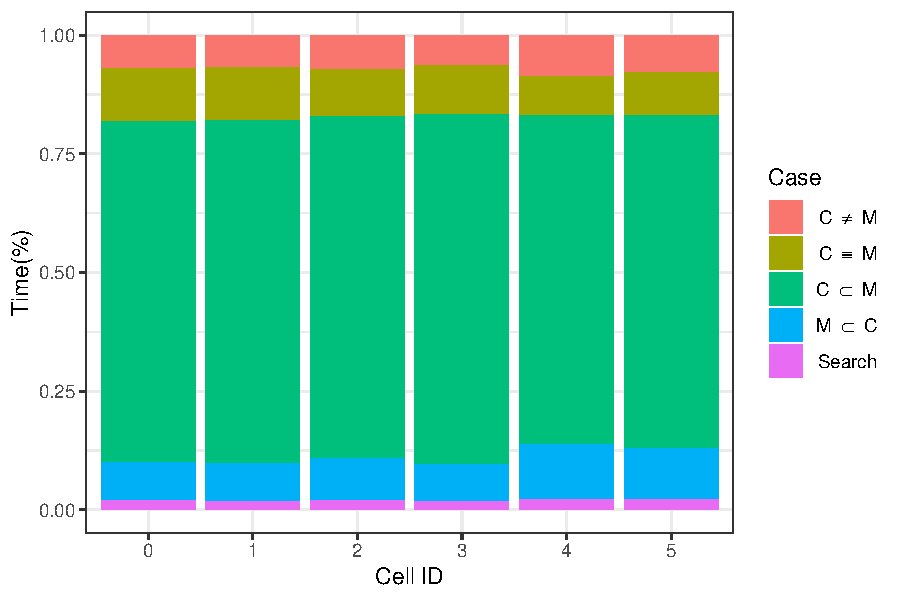
\includegraphics[width=\textwidth]{figures/Maximals/performanceBySum2}
        \end{minipage}
\end{frame}

\begin{frame}{Detecting maximal duplicates, subsets and supersets}
        {Average of time for each candidate to be evaluated...}
        \centering
        \begin{minipage}{0.49\textwidth}
                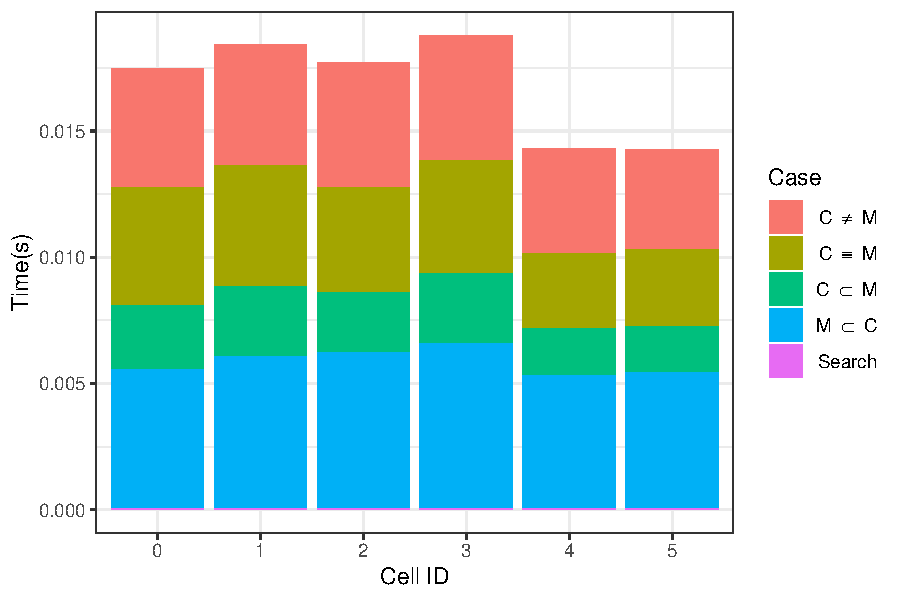
\includegraphics[width=\textwidth]{figures/Maximals/performanceByMean1}
        \end{minipage} %
        \begin{minipage}{0.49\textwidth}
                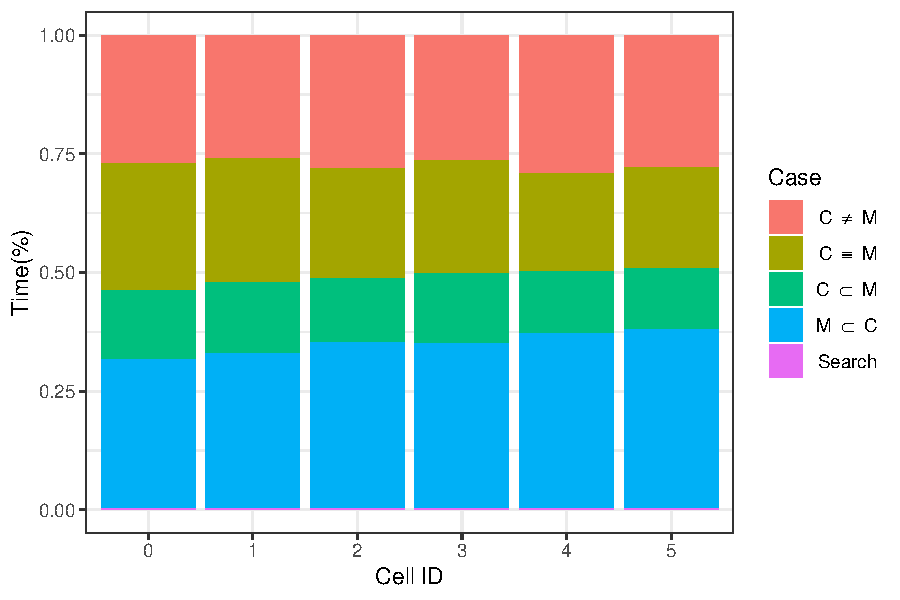
\includegraphics[width=\textwidth]{figures/Maximals/performanceByMean2}
        \end{minipage}
\end{frame}

\begin{frame}{Detecting maximal duplicates, subsets and supersets}
        \begin{table}[ht]
                \centering
                \begin{tabular}{rrrrr}
                        \toprule
                               & Number & Tree & Range & Position \\
                        Cell & candidates & size & size & found \\
                        \midrule
                        0 & 10393 & 258 & 170 & 77 \\
                        1 & 9579 & 231 & 167 & 84 \\
                        2 & 11994 & 276 & 166 & 78 \\
                        3 & 10765 & 251 & 170 & 87 \\
                        4 & 7974 & 204 & 123 & 64 \\
                        5 & 7936 & 188 & 126 & 61 \\
                        \bottomrule
                \end{tabular}
        \end{table}
\end{frame}

\begin{frame}{Detecting maximal duplicates, subsets and supersets}
    \centering
%    \includegraphics[width=0.6\textwidth]{figures/}
\end{frame}

\end{document}

